\chapter{世界面、威克转动与道对偶}

\lectureoverview{粒子描出一条世界线；弦则扫出一个世界面。对二者中任何一个进行量子化都需要对历史求和，但洛伦兹号差的求和是振荡的，难以定义。把世界面时间变为虚坐标后，得到一个由拉普拉斯方程支配的欧几里得理论。其共形对称性随即把四弦相互作用的裂缝状曲面变成带有四个边界插入点的圆盘，于是直接道与交叉道之间的对称性变得可见。}

\section{从世界线到对历史求和}

先从一个自由粒子开始。在非相对论力学中，它的位置是函数\(\mathbf x(t)\)，并且，在把质量取为1后，其作用量为
\begin{equation}
  S_{\mathrm{NR}}[\mathbf x]
  =\frac12\int_{t_1}^{t_2}\dot{\mathbf x}^{\,2}\,dt.
  \label{eq:l07-nr-action}
\end{equation}
对于相对论性描述，更自然的做法是把时间和空间放进一个矢量\(X^\mu(\tau)\)中，并沿轨迹用\(\tau\)参数化。相应的二次表达式为
\begin{equation}
  S_{\mathrm{rel}}[X]
  =\frac12\int_{\tau_1}^{\tau_2}
  \frac{dX^\mu}{d\tau}\frac{dX_\mu}{d\tau}\,d\tau.
  \label{eq:l07-rel-action}
\end{equation}
上指标与下指标编码了时间与空间之间的洛伦兹号差。
\editorialnote{这里使用的是在固定世界线参数化下的二次相对论作用量。显式重参数化不变的替代方案正比于固有长度，这一点在讲座后文会提到。}

\begin{figure}[H]
  \centering
  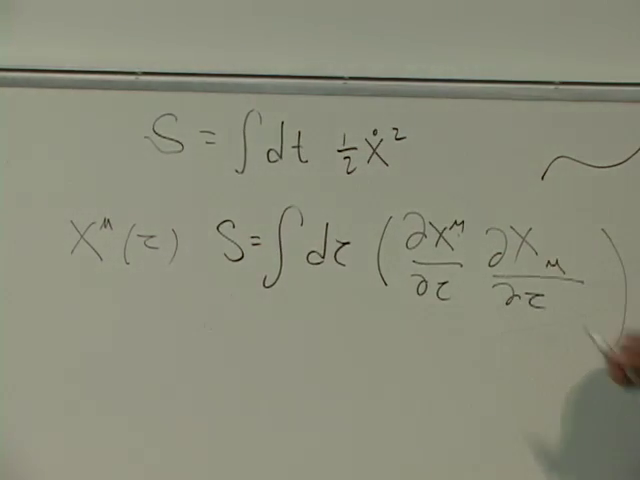
\includegraphics[width=0.72\textwidth]{lecture_07_figure_01.png}
  \caption{非相对论作用量及其相对论二次对应物一起写在黑板上。}
  \lectureframe{00:03:35}
  \label{fig:l07-particle-actions}
\end{figure}

在经典层面，人们固定端点并改变路径。自由粒子随后沿一条速度恒定的直线世界线运动。量子力学问的是另一个问题。它并不在端点之间选出一条轨迹；它问的是从一点出发并在另一点被探测到的振幅。每一条介于其间的路径都贡献一个相位，
\begin{equation}
  K(2,1)=\int_{X(1)}^{X(2)}\!\mathcal D X\,
  e^{iS[X]}.
  \label{eq:l07-feynman-integral}
\end{equation}
泛函积分是在无限维路径空间上的积分，而不是已经出现在作用量内部的普通积分。

\begin{figure}[H]
  \centering
  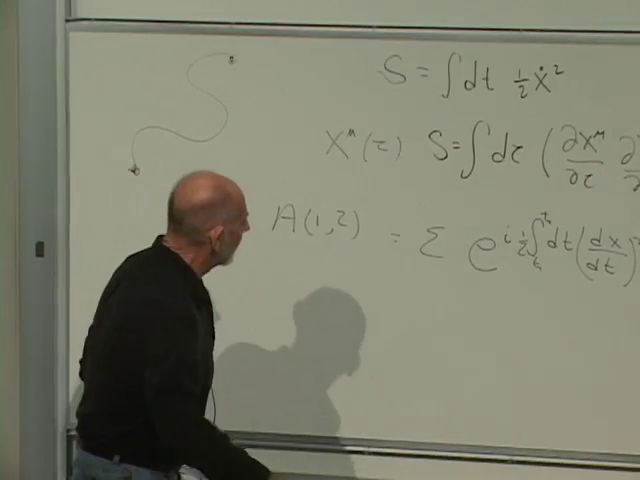
\includegraphics[width=0.72\textwidth]{lecture_07_figure_02.png}
  \caption{在取遍所有轨迹的求和之前，一条代表性路径以及赋予它的相位。}
  \lectureframe{00:06:21}
  \label{fig:l07-path-integral-board}
\end{figure}

用相对论语言来说，这个从点到点的振幅是一个传播子。对于相互作用，若干世界线段相遇。它们的作用量相加，相遇点被积分掉，并对外部粒子符合要求的图求和。因此，熟悉的费曼图展开已经隐含在对历史求和的指令之中。

符号\(S\)在这里将表示一个作用量。它既与熵无关，也与讲座接近末尾处使用的曼德尔施塔姆变量\(s\)无关。这种记号上的共用是传统使然，而非富有启发性。

\section{把时间转向侧面}

\eqref{eq:l07-feynman-integral}立刻存在一个问题。每个因子\(e^{iS}\)的模都是1。因此，一条剧烈振荡的轨迹和经典直线以相同的绝对权重进入；只有它们的相位不同。相消干涉恢复了经典行为，但这并不使形式积分成为一个普通的收敛对象。

通过
\begin{equation}
  \tau=\alpha s,
  \qquad
  d\tau=\alpha\,ds,
  \qquad
  \frac{dX}{d\tau}=\frac{1}{\alpha}\frac{dX}{ds}.
\end{equation}
引入一个新参数\(s\)。于是二次作用量按如下方式重新标度：
\begin{equation}
  \frac12\int d\tau
  \left(\frac{dX}{d\tau}\right)^2
  =
  \frac{1}{2\alpha}\int ds
  \left(\frac{dX}{ds}\right)^2.
  \label{eq:l07-rescaled-action}
\end{equation}
选择对应于\(\alpha=-i\)的围道会把振荡权重变为
\begin{equation}
  e^{iS}
  \longrightarrow
  \exp\!\left[-\frac12\int ds
  \left(\frac{dX}{ds}\right)^2\right]
  =e^{-S_E}.
  \label{eq:l07-euclidean-particle}
\end{equation}

\begin{figure}[H]
  \centering
  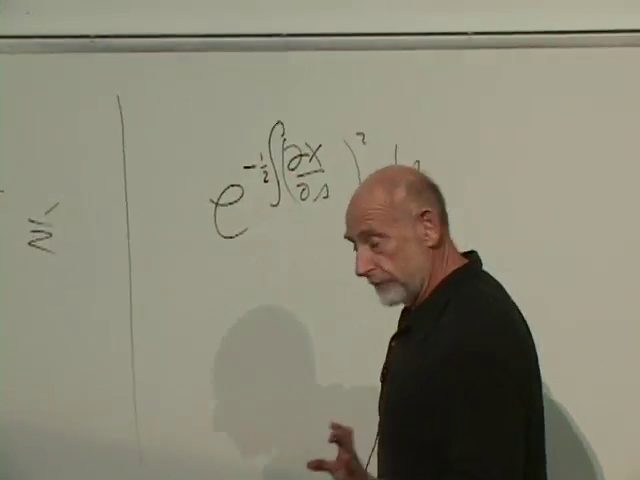
\includegraphics[width=0.66\textwidth]{lecture_07_figure_03.png}
  \caption{虚时间替换后的欧几里得粒子权重；指数为实且非正。}
  \lectureframe{00:16:20}
  \label{fig:l07-particle-wick}
\end{figure}

一条跑到很远再返回的路径，或者一条不跑远却快速扭动的路径，都有很大的正\(S_E\)，因而被指数压低。结果是一个维纳型积分，对此存在严格的收敛理论。从实\(\tau\)继承来的端点位于一条虚\(s\)围道上。实践中，人们在收敛区域内计算欧几里得对象，并把答案解析延拓回物理的洛伦兹变量。这一操作就是威克转动：时间是为了计算而被转向侧面，而不是被丢弃。

\section{从世界线到世界面}

点粒子有一条世界线。开弦扫出一条带子，闭弦扫出一根管子。坐标\((\sigma,\tau)\)标记这个二维世界面上的点，而
\begin{equation}
  X^\mu=X^\mu(\sigma,\tau)
  \label{eq:l07-embedding}
\end{equation}
给出被标记点的时空位置。知道所有函数\(X^\mu\)就完全确定了弦的整个历史。

二次洛伦兹世界面作用量具有与普通振动弦相同的动能减势能结构：
\begin{equation}
  S_{\mathrm{ws}}[X]
  =\frac{T_s}{2}\int d\tau\,d\sigma\,
  \left[
    \partial_\tau X^\mu\partial_\tau X_\mu
    -
    \partial_\sigma X^\mu\partial_\sigma X_\mu
  \right].
  \label{eq:l07-lorentzian-worldsheet}
\end{equation}
整体张力\(T_s\)固定了标度；本讲在专注于导数结构时将其略去。

\begin{figure}[H]
  \centering
  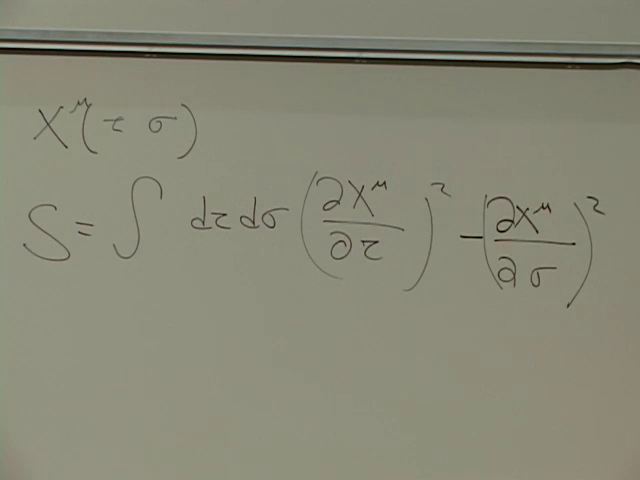
\includegraphics[width=0.72\textwidth]{lecture_07_figure_04.png}
  \caption{\(X^\mu(\sigma,\tau)\)的洛伦兹世界面作用量，及其动能减势能的符号。}
  \lectureframe{00:24:26}
  \label{fig:l07-worldsheet-action}
\end{figure}

弦振幅通过将此作用量指数化并对连接指定初末弦构型的所有曲面求和得到：
\begin{equation}
  \mathcal A=\int\mathcal D X\,e^{iS_{\mathrm{ws}}[X]}.
  \label{eq:l07-surface-integral}
\end{equation}
同一规则处理两弦变为两弦、两弦变为三弦，或任何其他允许的外腿构型。不同的世界面拓扑也属于该求和。添加洞是点粒子图展开中添加圈阶的弦对应物。

\begin{figure}[H]
  \centering
  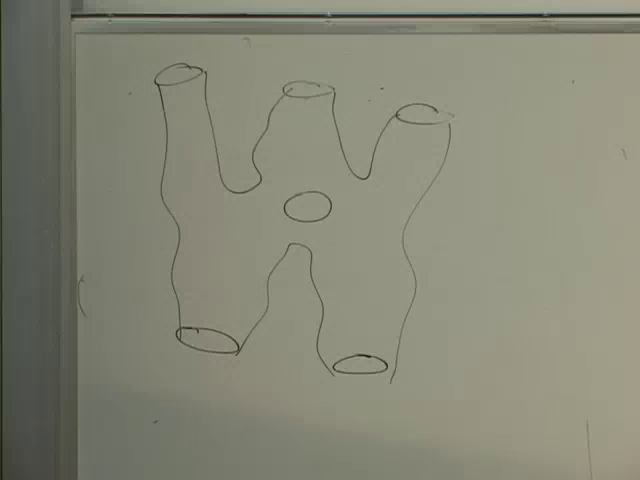
\includegraphics[width=0.66\textwidth]{lecture_07_figure_05.png}
  \caption{连接若干外弦的曲面，其中一个洞代表不同的世界面拓扑。}
  \lectureframe{00:27:14}
  \label{fig:l07-surface-topology}
\end{figure}

\begin{classroomqa}
\audiencequestion{对于点电子，\(\sigma\)导数是否直接消失？\lecturetimestamp{00:27:56}}
\lecturerresponse{点粒子首先就没有\(\sigma\)坐标。然而两幅图像是相联系的：当外态相对于弦标度很轻且过程能量很低时，弦振幅重现普通的点粒子费曼图。该极限不仅仅是把一个导数设为零。}
\end{classroomqa}

曲面积分与路径积分有相同的收敛问题。在对世界面时间做威克转动后，其稳定的欧几里得形式为
\begin{equation}
  \begin{aligned}
    S_{E,\mathrm{ws}}[X]
    &=\frac{T_s}{2}\int d\tau\,d\sigma\,
      \left[
        \partial_\tau X^\mu\partial_\tau X_\mu
        +\partial_\sigma X^\mu\partial_\sigma X_\mu
      \right],\\
    \mathcal A_E&=\int\mathcal D X\,e^{-S_{E,\mathrm{ws}}}.
  \end{aligned}
  \label{eq:l07-euclidean-worldsheet}
\end{equation}
两个导数现在都以相同的正号进入。剧烈振动或大幅拉伸的曲面具有大的欧几里得作用量并被压低。

\begin{figure}[H]
  \centering
  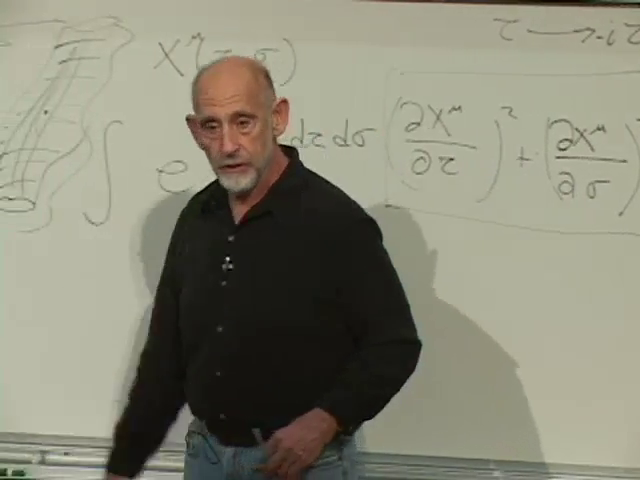
\includegraphics[width=0.72\textwidth]{lecture_07_figure_06.png}
  \caption{在\(\tau\)被转动到虚时间后的正欧几里得世界面密度。}
  \lectureframe{00:34:29}
  \label{fig:l07-worldsheet-wick}
\end{figure}

还有一种几何上直接的表述。可以给相对论性粒子赋予一个正比于其路径固有长度的作用量；可以给弦赋予一个正比于其世界面时空面积的作用量。后者即南部--后藤作用量。这里所用的二次世界面形式习惯上称为波利亚科夫形式，对当前计算要容易得多。
\editorialnote{本讲包含一段关于历史命名的幽默讨论，也提到了相关的刘维尔作用量和狄利克雷边界条件。该推导无需优先权主张：只用到面积表述与辅助度规表述的等价性。}

\section{欧几里得运动方程}

坐标\(\sigma\)和\(\tau\)只是世界面上的标签。因此下一个问题不可避免：哪些重标记使理论保持不变？答案最容易从运动方程看出。对\eqref{eq:l07-euclidean-worldsheet}变分，逐分量给出
\begin{equation}
  \partial_\tau^2X^\mu+\partial_\sigma^2X^\mu=0.
  \label{eq:l07-laplace}
\end{equation}
在威克转动之前，相对符号为负，这是一个波动方程。在欧几里得号差下两个符号都为正，因此它是二维拉普拉斯方程。

\begin{classroomqa}
\audiencequestion{这是振动鼓面的方程吗？
\lecturetimestamp{00:41:50}}
\lecturerresponse{它与之密切相关，但振动鼓面还带有一个真实时间坐标，因此服从波动方程。这里的方程是欧几里得拉普拉斯方程。无电荷区域中的静电势提供了一个更直接的熟悉例子。}
\end{classroomqa}

\begin{classroomqa}
\audiencequestion{作用量含有一阶导数。为什么其方程含有二阶导数？\lecturetimestamp{00:42:44}}
\lecturerresponse{对一阶导数的二次项变分并分部积分，会把一个导数移到该一阶导数上。这是场论版本的\(\dot x^{\,2}\)出现在作用量中而产生运动方程中的\(\ddot x\)。}
\end{classroomqa}

\begin{figure}[H]
  \centering
  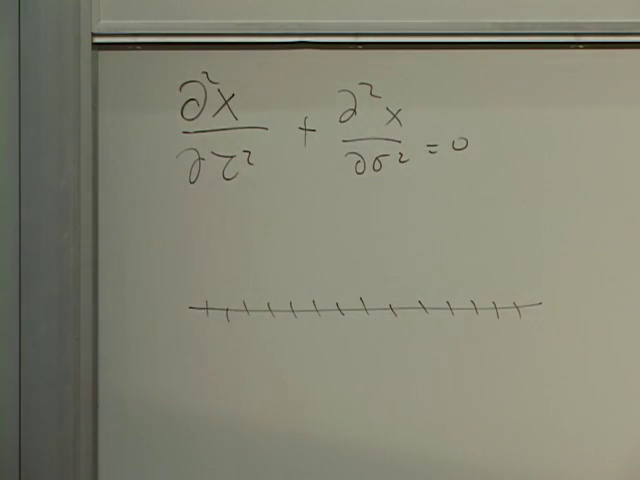
\includegraphics[width=0.68\textwidth]{lecture_07_figure_07.png}
  \caption{带正号的拉普拉斯方程，以及用于解释其二阶导数的第一行离散表达式。}
  \lectureframe{00:43:30}
  \label{fig:l07-laplace-board}
\end{figure}

为看清几何，先用间距\(\epsilon\)离散化一个坐标。一阶导数是相邻差分，而二阶导数是相邻差分之差：
\begin{equation}
  \frac{d^2X}{ds^2}\bigg|_{2}
  \longrightarrow
  \frac{X(3)-2X(2)+X(1)}{\epsilon^2}.
  \label{eq:l07-second-difference}
\end{equation}

\begin{figure}[H]
  \centering
  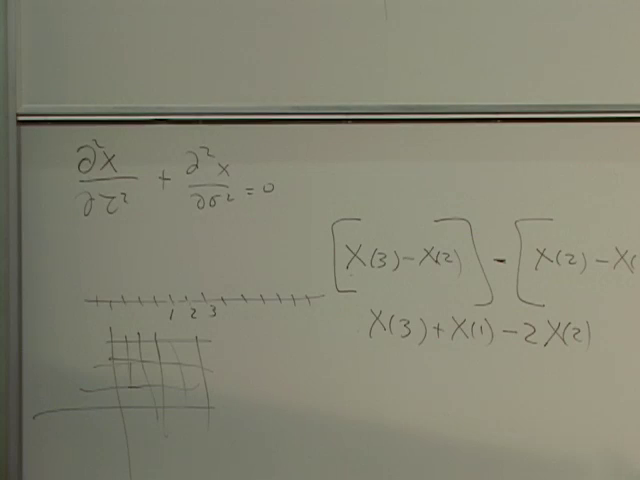
\includegraphics[width=0.72\textwidth]{lecture_07_figure_08.png}
  \caption{编号行、小点阵块，以及二阶导数的有限差分展开。}
  \lectureframe{00:45:51}
  \label{fig:l07-finite-difference-board}
\end{figure}

现在离散化\((\sigma,\tau)\)平面。将中心点\(5\)的四个最近邻标记为\(1,2,3,4\)。方程\eqref{eq:l07-laplace}变为
\begin{equation}
  X(1)+X(2)+X(3)+X(4)-4X(5)=0,
\end{equation}
或
\begin{equation}
  X(5)=\frac14\bigl[X(1)+X(2)+X(3)+X(4)\bigr].
  \label{eq:l07-mean-value}
\end{equation}

\begin{figure}[H]
  \centering
  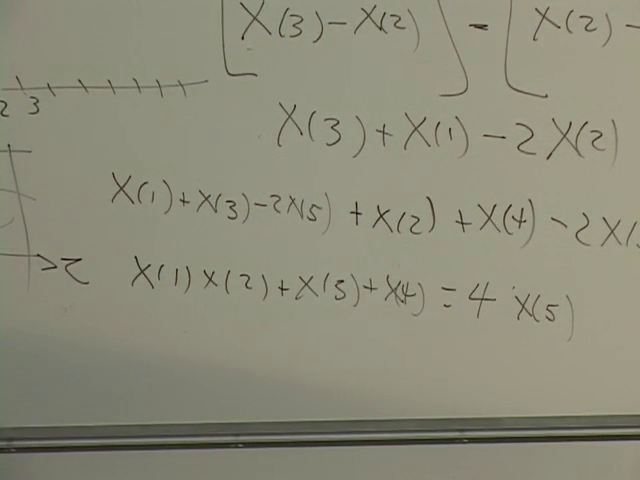
\includegraphics[width=0.72\textwidth]{lecture_07_figure_09.png}
  \caption{完成后的二维有限差分方程：中心值等于其四个相邻点的平均值。}
  \lectureframe{00:48:26}
  \label{fig:l07-mean-value-board}
\end{figure}

这一均值性质对任意取向的无穷小正方形都成立。它是拉普拉斯方程的局部几何内容，也是通向共形对称性的桥梁。

\section{共形坐标}

考虑从\((\sigma,\tau)\)到\((\sigma',\tau')\)的变换。一般的形变会把一个小正方形变为任意四边形。这里相关的特殊变换则把每个无穷小正方形变为另一个无穷小正方形，可能带有旋转和缩放。等价地说，它们保持曲线相交处的角度。这些就是共形变换。

\begin{figure}[H]
  \centering
  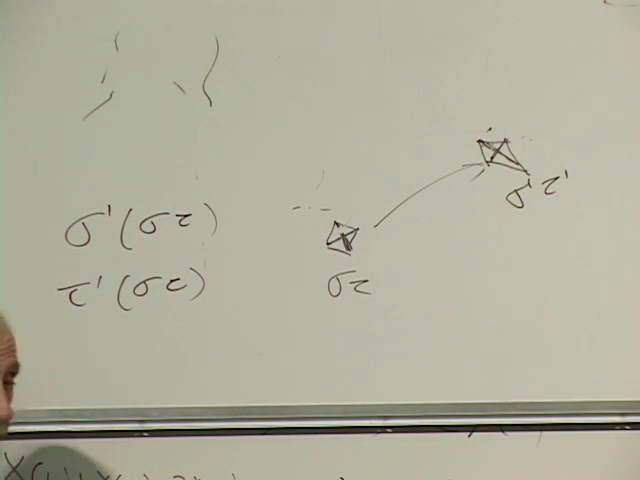
\includegraphics[width=0.68\textwidth]{lecture_07_figure_10.png}
  \caption{一个局部正方形被映射为另一个小图形，同时检验其角度是否被共形地保持。}
  \lectureframe{00:53:25}
  \label{fig:l07-conformal-board}
\end{figure}

\begin{classroomqa}
\audiencequestion{如果角度被保持，那么该变换基本上只是旋转吗？\lecturetimestamp{00:53:31}}
\lecturerresponse{只在局部如此，而且即便在局部，也允许一个共同的尺度变化。局部的旋转和尺度因子可以逐点变化，因此坐标网格可以弯曲，在一个区域膨胀，在另一个区域收缩，同时保持无穷小形状。}
\end{classroomqa}

保角映射不必保持大小。如果大小也在各处固定，那么可能性就会坍缩为小得多的刚性类，即平移和旋转。共形映射则保持局部形状。这就是为什么地图投影可以保持一个小岛的形状，却极大地扭曲其面积。

\begin{classroomqa}
\audiencequestion{共形映射等价于说坐标系是平坦的吗？\lecturetimestamp{00:55:35}}
\lecturerresponse{不。平坦性和共形性是两种不同的陈述。共形映射可以使用弯曲的坐标线；它所保持的是相交曲线之间的角度。墨卡托型地图投影就是一个熟悉的例子，它在保持局部形状的同时具有显著的尺度畸变。}
\end{classroomqa}

在二维情形中，所需的变换局部地由复坐标的解析函数生成
\begin{equation}
  z=\sigma+i\tau.
\end{equation}
有限边界可以显著改变外观。一个正方形区域可以被映射为一个光滑区域，原来的角被送到新边界上的普通点，而不是其视觉上突出的点。这并不矛盾：共形性是局部的内部条件，而映射在其正则之处保持无穷小角度。

\begin{classroomqa}
\audiencequestion{这种坐标自由度是否就是先前那个
join--split图可以被选为对称形式的原因？
\lecturetimestamp{00:56:32}}
\lecturerresponse{是的。正是这种保持世界面方程的共形自由度，让我们能够把别扭的相互作用带替换为更对称的区域。剩余的自由度并不会移除物理的
join--split参数；它只是把该参数重新包装为边界插入点的相对位置。}
\end{classroomqa}

\section{带缝薄片与圆盘}

回到四弦散射。两条开弦进入，它们的端点相接，合并后的弦传播，随后又分裂。画成平坦世界面时，这一过程是一条从两端被切开的无限长条带。两条缝的尖端之间的间隔\(\tau_0\)是中间弦的寿命，而振幅对它积分。

\begin{figure}[H]
  \centering
  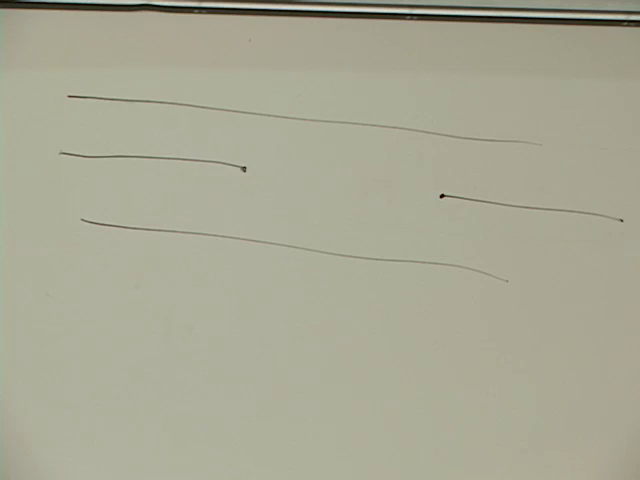
\includegraphics[width=0.72\textwidth]{lecture_07_figure_11.png}
  \caption{表示两条开弦相接、共同传播并再次分裂的双缝长条带。}
  \lectureframe{01:00:20}
  \label{fig:l07-slit-strip}
\end{figure}

欧几里得化之后，这一区域上的嵌入场满足拉普拉斯方程。因此共形不变性允许把带缝长条带映射为圆盘。看清其拓扑的一种方式是用同心圆叶状分层圆盘，并连续形变这些闭合曲线，直到它们填满带缝区域。无穷远处的端点在映射下成为特殊的边界点。

\begin{figure}[H]
  \centering
  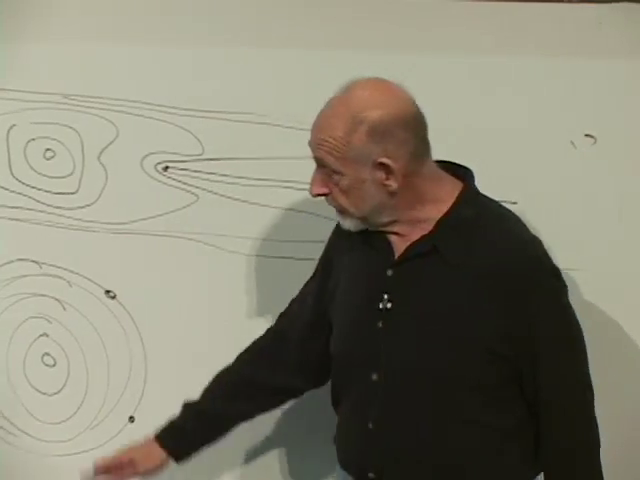
\includegraphics[width=0.72\textwidth]{lecture_07_figure_12.png}
  \medskip

  \begin{adjustbox}{max width=\linewidth}
  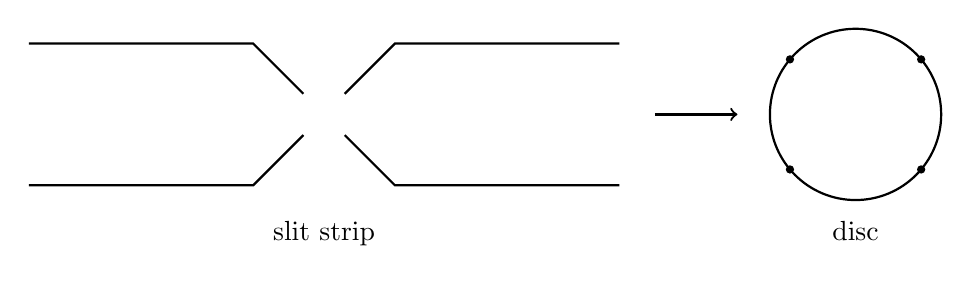
\begin{tikzpicture}[x=0.75cm,y=0.75cm]
    \draw[thick] (-5,1.2) -- (-1.2,1.2) -- (-0.35,0.35);
    \draw[thick] (-5,-1.2) -- (-1.2,-1.2) -- (-0.35,-0.35);
    \draw[thick] (0.35,0.35) -- (1.2,1.2) -- (5,1.2);
    \draw[thick] (0.35,-0.35) -- (1.2,-1.2) -- (5,-1.2);
    \draw[->,thick] (5.6,0) -- (7.0,0);
    \draw[thick] (9.0,0) circle (1.45);
    \foreach \a in {40,140,220,320} \fill (9.0,0) ++(\a:1.45) circle (1.5pt);
    \node[below] at (0,-1.65) {slit strip};
    \node[below] at (9.0,-1.65) {disc};
  \end{tikzpicture}
  \end{adjustbox}
  \caption{黑板上的等值线比较，以及从带缝长条带到圆盘的共形映射的清晰示意图。四个外部端点成为四个特殊的边界点。}
  \lectureframe{01:04:46}
  \label{fig:l07-strip-to-disc}
\end{figure}

外部态在这种坐标变换中并未丢失。动量、粒子类型和振子能级必须插入到四个特殊点上。承载这些信息的形式对象是顶点算子。它们的详细构造留待以后，但其作用已经清楚：它们把原本均匀的世界面路径积分变为一个指定的散射实验。

在利用圆盘的共形变换将三个边界点移到方便的参考位置之后，还剩下一个实相对位置。它可以由四个有序边界点的交比来表示。这就是旧的寿命\(\tau_0\)的圆盘版本。

\begin{figure}[H]
  \centering
  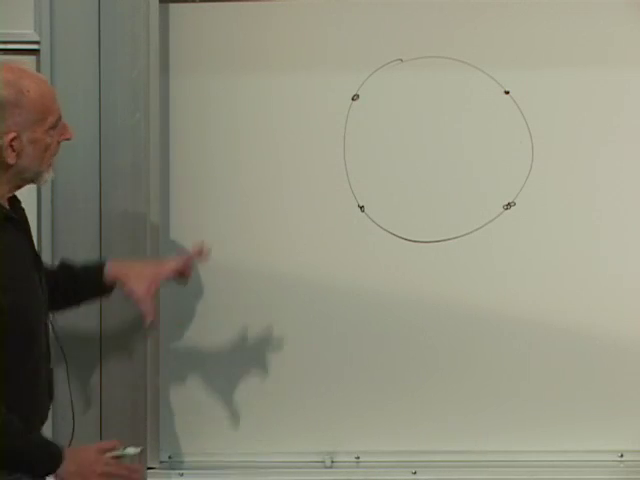
\includegraphics[width=0.62\textwidth]{lecture_07_figure_13.png}
  \caption{圆盘边界上的四个插入点。共形自由度除去了它们有序位形中除一个实模数之外的全部模数。}
  \lectureframe{01:10:55}
  \label{fig:l07-four-points}
\end{figure}

因此寿命积分并没有消失。它变成了对那个剩余模数的积分。采用惯用坐标\(0<z<1\)，四点开弦积分取与上一讲中所得相同的形式，
\begin{equation}
  \mathcal A(s,t)\propto
  \int_0^1 z^{-s-1}(1-z)^{-t-1}\,dz.
  \label{eq:l07-modulus-integral}
\end{equation}

\section{同一个曲面的两个极限}

在模空间的一端，与入射对相关联的两个插入点彼此靠近。在缝条坐标中，这是连接与分裂之间的一段长间隔：一个直接道中间弦传播了很长时间。在另一端，另一对相邻的点彼此靠近。同一个曲面于是自然地被读作交叉道交换。这些描述在条带上看起来互不相关，但它们是一个圆盘积分的相邻边界极限。

回到上一讲的mostly-plus约定，
\begin{equation}
  -s=(k_1+k_2)^2,
  \qquad
  -t=(k_1+k_3)^2.
  \label{eq:l07-mandelstam}
\end{equation}
直接极限将极点组织在\(s\)中；交叉极限将极点组织在\(t\)中。
\editorialnote{在讲座接近尾声时，黑板上对Mandelstam不变量使用了简写符号，同时将\(s\)等同于正的中心-of-mass能量平方。方程\eqref{eq:l07-mandelstam}保持了第6讲中确立的mostly-plus约定。}

\begin{figure}[H]
  \centering
  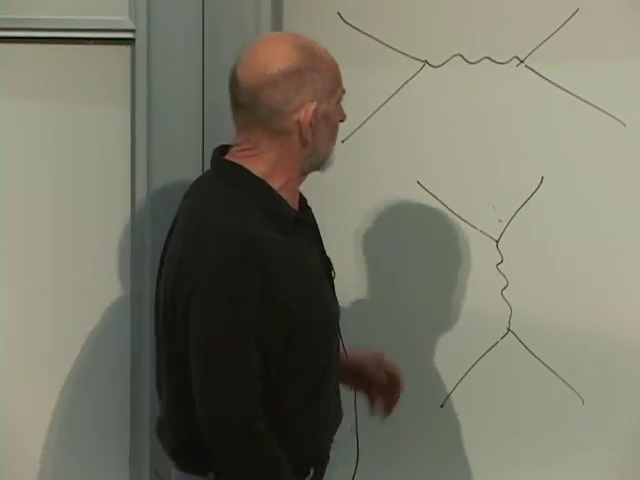
\includegraphics[width=0.62\textwidth]{lecture_07_figure_14.png}
  \caption{两个道图：在一个取向上是长传播，在交叉取向上是交换。}
  \lectureframe{01:19:27}
  \label{fig:l07-channel-diagrams}
\end{figure}

\begin{figure}[H]
  \centering
  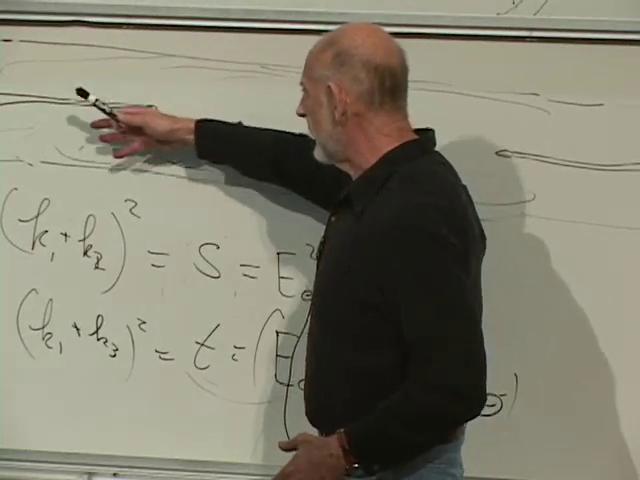
\includegraphics[width=0.72\textwidth]{lecture_07_figure_15.png}
  \caption{黑板回到\(s\)道和\(t\)道的动量配对，同时比较圆盘模数的两个极限。}
  \lectureframe{01:19:40}
  \label{fig:l07-st-board}
\end{figure}

因此一个解析对象同时提供了两种展开：
\begin{equation}
  \mathcal A(s,t)=\mathcal A(t,s).
\end{equation}
这就是道对偶。在最初的共振语言中，对直接道态求和竟也能编码交叉道交换，这显得不可思议。在欧几里得世界面上，共形对称性解释了为什么这两种描述属于同一个曲面。历史上，这一解释在Veneziano振幅于1969年被发现之后很快就出现了。

\begin{classroomqa}
\audiencequestion{是否也存在对应于交叉取向的缝条图像？\lecturetimestamp{01:20:49}}
\lecturerresponse{是的，但被称为时间的方向必须另行选取。同一个欧几里得曲面可以被切片，使得另一对外部端点位于遥远的过去和未来。正是这种替代切片方式，使得单个世界面允许多于一种道的解释。}
\end{classroomqa}

\begin{classroomqa}
\audiencequestion{弦保持连接的时间是否由耦合常数决定？\lecturetimestamp{01:21:39}}
\lecturerresponse{不会选出任何固定的寿命。寿命是一个积分变量，每一个值都有贡献。耦合控制连接与分裂的权重---等价地，即衰变强度---，并以相乘的方式进入振幅；它并不取代模数积分。}
\end{classroomqa}
